\documentclass[xcolor=dvipsnames]{beamer}
\usepackage{lmodern}
\usepackage[T1]{fontenc}
\usepackage[english]{babel}
\usepackage[utf8]{inputenc}

\usepackage{manfnt}
\usepackage{wasysym}
\usepackage{listings}
\usepackage{graphicx}
\usepackage{url}
\usepackage{ulem}
\usepackage{marvosym}
\usepackage{skull}
\usepackage{proof}
\usepackage{array}
\usepackage{colortbl}
\usepackage{xspace}
\setbeamertemplate{navigation symbols}{}

\title[Thesis Proposal]{{\bf Practical Concurrency Testing}}
\subtitle[]{a thesis proposal}
\author[Ben Blum]{Ben Blum \texttt{(bblum@cs.cmu.edu)}}

\institute[CMU CSD]{Carnegie Mellon University}
\date[]{2017, April 25}

\setbeamertemplate{footline}{\hspace*{.5cm}\scriptsize{\insertauthor\hspace*{50pt} \hfill\insertframenumber\hspace*{.5cm}}} 

\usecolortheme{seahorse}
\usecolortheme{rose}
\useoutertheme{infolines}

\usecolortheme[named=ForestGreen]{structure}

\newcommand\noob{\mathsf{noob}}
\newcommand\gibs{\mathsf{gibs}}
\newcommand\dps{\mathsf{dps}}
\newcommand\squig\rightsquigarrow
\newcommand\Coloneqq{\mathrel{\mathop{::}}=}
\newcommand\dmg{\text{\Laserbeam}}
\newcommand\delter\delta
\newcommand\alpher\alpha
\newcommand\defnor{\text{ }|\text{ }}

\newcommand\pimp{\mathop{\supset}}
\newcommand\pand{\mathop{\wedge}}
\newcommand\por{\mathop{\vee}}
\newcommand\ptrue{\top}
\newcommand\pfalse{\bot}

\newcommand\hilight[2]{\color{#1}#2\color{black}}
\definecolor{olivegreen}{RGB}{0,127,0}

\begin{document}
%\renewcommand{\inserttotalframenumber}{39}
\normalem
\begin{frame}
	\titlepage
\end{frame}

%%%%%%%%%%%%%%%%%%%%%%%%%%%%%%%%%%%%%%%%%%%%%%%%%%%%%%%%%%%%%%%%%%%%%%%%%%%%%%%%
%%%%%%%%%%%%%%%%%%%%%%%%%%%%%%%%%%%%%%%%%%%%%%%%%%%%%%%%%%%%%%%%%%%%%%%%%%%%%%%%
%%%%%%%%%%%%%%%%%%%%%%%%%%%%%%%%%%%%%%%%%%%%%%%%%%%%%%%%%%%%%%%%%%%%%%%%%%%%%%%%

\newcommand\linegap{\vspace{0.2in}}
\newcommand\breakslide[1]{\begin{frame}{} \begin{center} #1 \end{center} \end{frame}}

\section{Introduction}
\subsection{Motivation}

\begin{frame}{Thesis Statement}
	Thanks to the new algorithms, heuristics, and concurrency models I have developed,
	stateless model checking is an appropriate and accessible concurrency testing technique
	for programmers in both educational and real-world settings.
\end{frame}

\begin{frame}{Outline}
	guess i should outline my talk huh
\end{frame}


%%%%%%%%%%%%%%%%%%%%%%%%%%%%%%%%%%%%%%%%%%%%%%%%%%%%%%%%%%%%%%%%%%%%%%%%%%%%%%%%
%%%%%%%%%%%%%%%%%%%%%%%%%%%%%%%%%%%%%%%%%%%%%%%%%%%%%%%%%%%%%%%%%%%%%%%%%%%%%%%%
%%%%%%%%%%%%%%%%%%%%%%%%%%%%%%%%%%%%%%%%%%%%%%%%%%%%%%%%%%%%%%%%%%%%%%%%%%%%%%%%

\section{some kinda introductory}

%\begin{frame}{overview of state of art}
%	\begin{itemize}
%		\item so like, you got all this threads, right?
%		\item n then you just make em go any which way
%		\item see what all bugs come out
%	\end{itemize}
%\end{frame}

%%%%%%%%%%%%%%%%%%%%%%%%%%%%%%%%%%%%%%%%%%%%%%%%%%%%%%%%%%%%%%%%%%%%%%%%%%%%%%%%
%%%%%%%%%%%%%%%%%%%%%%%%%%%%%%%%%%%%%%%%%%%%%%%%%%%%%%%%%%%%%%%%%%%%%%%%%%%%%%%%
%%%%%%%%%%%%%%%%%%%%%%%%%%%%%%%%%%%%%%%%%%%%%%%%%%%%%%%%%%%%%%%%%%%%%%%%%%%%%%%%

\section{Education}

\breakslide{\Large Educational Use}

\begin{frame}{Pebbles}
	CMU (15-410)
	\linegap

	Kernel (``P3'')
	\begin{itemize}
		%\item UNIX-like educational kernel specification
		\item Students implement scheduler, synchronization, VM %from scratch %% trying not to be too arrogant ._.
		\item UNIX-like process lifecycle ({\tt fork}, {\tt exec}, {\tt vanish}, {\tt wait})
		%\item Teams of 2
		\item Testing with MC requires manual annotation {\em [Blum '12]}
	\end{itemize}
	\pause
	\linegap

	Thread library (``P2'')
	\begin{itemize}
		\item POSIX-like userspace thread library %(also teams of 2)
		\item Students provided reference Pebbles implementation
		\item Fixed APIs $\rightarrow$ instrumentation can be automated
		\item May still need heuristics to handle ad-hoc synchronization
	\end{itemize}
\end{frame}

\begin{frame}{15-410 User Study}
	Method (since spring 2015)
	\begin{itemize}
		\item Guest lecture midway during P2
		\item Landslide (+ Quicksand) provided with 6 test cases and user guide
		\item Student code snapshots and bugs found recorded each use
	\end{itemize}
	\pause
	\linegap

	Results (as of spring 2016)
	\begin{itemize}
		\item 47/90 groups volunteered
		\item 85 concurrency bugs found; 53 which students then fixed
		\item No visible impact on ultimate grades...
	\end{itemize}
\end{frame}

\begin{frame}{15-410 User Study - Grades Results} % lack thereof
	\begin{center}
		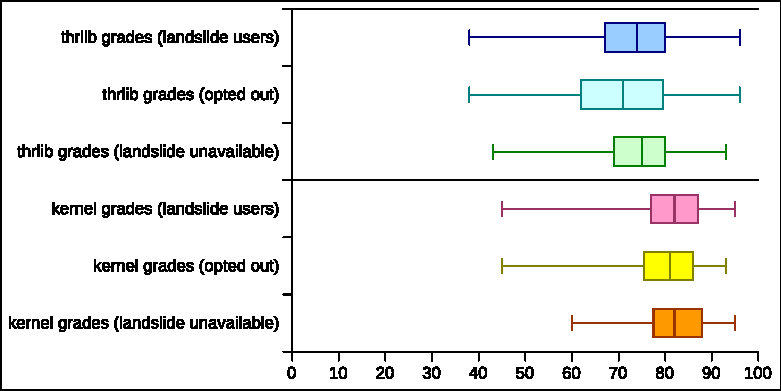
\includegraphics[width=\textwidth]{../p2-p3-distribution.pdf}
	\end{center}
\end{frame}

%%%%

\begin{frame}{Pintos}
	U. of Chicago (CMSC 23000), Berkeley (CS162), Stanford (CS140)
	\linegap

	Kernel (``threads'')
	\begin{itemize}
		\item Students implement priority scheduling, sleep
		\item Basecode provides round-robin scheduler, synchronization
	\end{itemize}
	\linegap

	Processes (``userprog'')
	\begin{itemize}
		\item UNIX-like process lifecycle ({\tt exec}, {\tt exit}, {\tt wait})
		\item File descriptor management ({\tt create}, {\tt remove}, {\tt open}, {\tt read}, ...)
	\end{itemize}
	\linegap

	VM, filesys projects not as concurrency-focused as above
\end{frame}

\begin{frame}{Pintos \& Landslide}
	Existing support:
	\begin{itemize}
		\item Lockset/vector-clock analyses extended to interrupt-disabling
		\item Automatically inserting (most) kernel annotations
		%\item (various engineering challenges) % palloc heap, non-direct-mapped kernelspace, skipping driver init loops
		\item Often requires manual intervention
	\end{itemize}
	% "Works enough for OOPSLA but not enough for the studence"
	\linegap

	Still needed:
	\begin{itemize}
		\item Improved automation to support corner-case student designs
		\item More concurrency test cases
		\item Remove proprietary Simics dependence by porting to Bochs
	\end{itemize}
\end{frame}

\begin{frame}{Deliverables}
	Pebbles
	\begin{itemize}
		\item Discuss factors keeping Landslide from improving grades
		%\item Discuss how to make P3 and Landslide compromise to work together
		\item Study accuracy of automation heuristics
	\end{itemize}
	\linegap

	Pintos
	\begin{itemize}
		\item Open-source port of Landslide to Bochs
		\item 2 semesters of user study in Pintos class(es)
		\item Compare incidence/nature of bugs found to Pebbles
	\end{itemize}
	\linegap
\end{frame}

%%%%%%%%%%%%%%%%%%%%%%%%%%%%%%%%%%%%%%%%%%%%%%%%%%%%%%%%%%%%%%%%%%%%%%%%%%%%%%%%
%%%%%%%%%%%%%%%%%%%%%%%%%%%%%%%%%%%%%%%%%%%%%%%%%%%%%%%%%%%%%%%%%%%%%%%%%%%%%%%%
%%%%%%%%%%%%%%%%%%%%%%%%%%%%%%%%%%%%%%%%%%%%%%%%%%%%%%%%%%%%%%%%%%%%%%%%%%%%%%%%

\section{Transactional Memory}
\newcommand\xbegin{\texttt{\_xbegin()}\xspace}
\newcommand\xend{\texttt{\_xend()}\xspace}
\newcommand\xabort{\texttt{\_xabort()}\xspace}

\breakslide{\Large Transactional Memory}

\begin{frame}{Example}
	\begin{center}
		\begin{tabular}{l}
			\texttt{if ((status = \_xbegin()) == \_XBEGIN\_STARTED) \{} \\
			%\texttt{} \\
			%\texttt{} \\
			\texttt{~~~~foo++;} \\
			\texttt{~~~~\_xend();} \\
			\texttt{\} else \{}\\ %if (status != \_XABORT\_EXPLICIT) \{} \\
			\texttt{~~~~mutex\_lock(\&foo\_lock);} \\
			\texttt{~~~~foo++;} \\
			\texttt{~~~~mutex\_unlock(\&foo\_lock);} \\
			\texttt{\}} \\
		\end{tabular}
	\end{center}
\end{frame}

\begin{frame}{HTM Execution Semantics}
	Attempting a transaction
	\begin{itemize}
		\item Code between \xbegin and \xend is provisionally executed
		\item All writes kept in cache until \xend
		\item \xend commits changes atomically (w.r.t. other CPUs)
	\end{itemize}
	\pause
	\linegap

	Transaction failure
	\begin{itemize}
		\item Possible reasons:
			\begin{itemize}
				\item Memory conflict with another thread
				\item False sharing (conflict on same cache-line)
				\item Cache eviction, random interrupt, ...
			\end{itemize}
		\item Changes discarded, local state reverted, \xbegin returns failure
		\item {\tt else} branch runs some user-supplied backup plan
	\end{itemize}
\end{frame}

\begin{frame}{Model Checking Transactional Programs}
	What does it mean to MC a program?
	\begin{itemize}
		\item Capture all sites of nondeterminism as ``branch points'' %in a state space
		\item Control nondeterminism to force each possibility at each point
		\item (Identify equivalences to prune unnecessary branch points)
	\end{itemize}
	\pause
	\linegap

	MCing a transactional program
	\begin{itemize}
		\item Simulate TM, interleaving transactions, rolling-back upon conflicts
			\begin{itemize}
					% TODO: need a bonus slide to justify why this
					% imagine a pair of transactions each with multiple conflicting accesses
					% they should be treated as atomic
				\item slow; invites state space explosion
			\end{itemize}
		\item Enforce atomicity via scheduler, anticipate aborts via analysis
			\begin{itemize}
				\item (under HTM, all transactions might abort)
					% TODO: need a bonus slide on finding when a STM txn may abort.
			\end{itemize}
		\item Suffices to enumerate all {\em observationally-equivalent} schedules.
	\end{itemize}
\end{frame}

\begin{frame}{Concurrency model}
	What are a transactional program's {\em observable} behaviours?
	\begin{itemize}
		\item Transactional writes, if successful, appear atomically %to other threads
		\begin{itemize}
			\item Equivalent to a lock protecting that state
		\end{itemize}
			\pause
		\item Simultaneous transactions succeed only if no conflicts
		\begin{itemize}
			\item Equivalent (modulo performance) to serialize independent transactions
		\end{itemize}
			\pause
		\item Failing transactions' effects rolled-back with no trace
		\begin{itemize}
			\item Treat each \xbegin as a failure injection point
		\end{itemize}
	\end{itemize}
\end{frame}

\begin{frame}{Failure Injection - 2 dimensions of concurrency}
	% TODO - pict of mario man
\end{frame}

\begin{frame}{Deliverables}
	In the thesis, I will:
	\begin{itemize}
		\item Implement the HTM(-equivalent) concurrency model in Landslide
		\item Extend the model to support STM
		\item Prove equivalence to HTM/STM semantics % under MC
		\item Bugfind/verify a suite of unit tests \& real-world TM programs
	\end{itemize}
\end{frame}

%%%%%%%%%%%%%%%%%%%%%%%%%%%%%%%%%%%%%%%%%%%%%%%%%%%%%%%%%%%%%%%%%%%%%%%%%%%%%%%%
%%%%%%%%%%%%%%%%%%%%%%%%%%%%%%%%%%%%%%%%%%%%%%%%%%%%%%%%%%%%%%%%%%%%%%%%%%%%%%%%
%%%%%%%%%%%%%%%%%%%%%%%%%%%%%%%%%%%%%%%%%%%%%%%%%%%%%%%%%%%%%%%%%%%%%%%%%%%%%%%%

\section{End}

\begin{frame}{Timeline}
	\begin{itemize}
		\item 2017 Mar-Aug: Port Landslide to Bochs for Pintos
		\item 2017 Mar-Aug: Transactional memory
		\item 2017 Aug-Oct: Pintos user study
		\item 2017 Oct-Nov: Pebbles user study (again)
		\item 2017 Dec:     Start writing thesis
		\item 2018 Jan-Apr: More writing \& miscellany
		\item 2018 Feb-Mar: Pintos \& Pebbles (again)
		\item 2018 Apr-May: Defend \& graduate
	\end{itemize}
\end{frame}

\breakslide{\Large Q\&A
%\linegap
%
%\begin{center}
%	\includegraphics[width=0.65\textwidth]{3word-questions.png}
%\end{center}
}

%%%%%%%%%%%%%%%%%%%%%%%%%%%%%%%%%%%%%%%%%%%%%%%%%%%%%%%%%%%%%%%%%%%%%%%%%%%%%%%%
%%%%%%%%%%%%%%%%%%%%%%%%%%%%%%%%%%%%%%%%%%%%%%%%%%%%%%%%%%%%%%%%%%%%%%%%%%%%%%%%
%%%%%%%%%%%%%%%%%%%%%%%%%%%%%%%%%%%%%%%%%%%%%%%%%%%%%%%%%%%%%%%%%%%%%%%%%%%%%%%%

\section{Bonus Slides}

\begin{frame}{HTM: Even more dimensions of nondeterminism}
	% The gotcha: When xbegin can fail, it can emit diff error codes, which depend on what happened within.
	\begin{center}
		\begin{tabular}{l}
			\texttt{if ((status = \_xbegin()) == \_XBEGIN\_STARTED) \{} \\
			\texttt{~~~~if (foo < 100)}\\
			\texttt{~~~~~~~~\_xabort();} \\
			\texttt{~~~~foo++;} \\
			\texttt{~~~~\_xend();} \\
			\texttt{\} else if (status != \_XABORT\_EXPLICIT) \{} \\
			\texttt{~~~~mutex\_lock(\&foo\_lock);} \\
			\texttt{~~~~foo++;} \\
			\texttt{~~~~mutex\_unlock(\&foo\_lock);} \\
			\texttt{\}} \\
		\end{tabular}
	\end{center}
	\linegap

	\xbegin can fail with multiple possible error codes
	\begin{itemize}
		\item MC will identify on-the-fly when (e.g.) {\tt \_XABORT\_EXPLICIT} is possible
		\item Treat such transactions as having multiple failure injection possibilities
			% XXX: How to identify when the failure status is never used? Dataflow analysis?
	\end{itemize}
\end{frame}

\begin{frame}{HTM: Possible \xabort error codes}
	From GCC 4.8.2 manual \S 6.56.8, ``X86 transaction memory intrinsics'':
	\begin{itemize}
		\item {\tt \_XABORT\_EXPLICIT} - Transaction explicitely [sic] aborted with \xabort.
			%The parameter passed to \xabort is available with {\tt \_XABORT\_CODE(status)}
		\item {\tt \_XABORT\_RETRY} - Transaction retry is possible.
		\item {\tt \_XABORT\_CONFLICT} - Transaction abort due to a memory conflict with another thread
		\item {\tt \_XABORT\_CAPACITY} - Transaction abort due to the transaction using too much memory
		\item {\tt \_XABORT\_DEBUG} - Transaction abort due to a debug trap
		\item {\tt \_XABORT\_NESTED} - Transaction abort in a inner nested transaction 
	\end{itemize}
\end{frame}

\end{document}
